\documentclass[12pt]{article}
\usepackage{amsmath}
\usepackage{graphicx}
\usepackage{siunitx}
\usepackage{float}
\usepackage{geometry}
\geometry{margin=1in}
% used packages in the template
% import your package here 
\usepackage[utf8]{inputenc}
\usepackage{multicol}
\usepackage{xcolor}
\usepackage{subfigure}
\usepackage{siunitx}
%
\usepackage[utf8]{inputenc}
\usepackage{graphicx}
\usepackage{titlesec}
\usepackage[bookmarks,breaklinks,colorlinks=true,allcolors=blue]{hyperref}
\usepackage{listings}
\usepackage{inconsolata}
\usepackage{float}
\usepackage{eso-pic}
\usepackage[framemethod=tikz]{mdframed}

\usepackage[square,numbers]{natbib}
\AtBeginDocument{
  \renewcommand{\bibsection}{\chapter{\bibname}}
} % Bibliography in numbered chapter

\usepackage{geometry}
\usepackage{amsmath}
\usepackage{parskip}
\usepackage[official]{eurosym}
\setlength {\marginparwidth }{2cm} 
\usepackage{todonotes}
\usepackage{csquotes}

\usepackage{rotating}
\usepackage{lmodern}
\usepackage{setspace}
\usepackage{pdfpages}
\usepackage{svg}
\usepackage{listings}
\usepackage{xcolor}
\lstset{
  language=Python,
  basicstyle=\ttfamily\small,
  keywordstyle=\color{blue},
  commentstyle=\color{gray},
  stringstyle=\color{orange},
  showstringspaces=false,
  breaklines=true,
  frame=single,
  captionpos=b,
  tabsize=4

\begin{document}

% Title Page etc (unchanged preamble and title page)

% Title Page
\begin{titlepage}
  \begin{center}
    \vspace*{1cm}
    
\includegraphics[width=0.35\textwidth]{images/cedtnew.png}\\[0.5cm]
    {\Large \textbf{Centre for Electronic Design and Technology}}\\[0.25cm]
    {\large Netaji Subhas University of Technology, New Delhi}
    \vfill
    {\Huge \textbf{Curdling Experiment}}\\[0.3cm]
    \vspace{1.5cm}
    {\large \textbf{Submitted by}}\\[0.2cm]
    {\large Ansh Gupta and Shubham}\\
    \vspace{0.8cm}
    {\large \textbf{Date:} June 2024}
    \vspace*{1cm}
  \end{center}
\end{titlepage}

\clearpage
\pagenumbering{roman}
\tableofcontents
\newpage

% ------------------------------
\section{Synopsis}
This experiment aimed to monitor the temperature profile of milk during the curdling process to test the hypothesis that curdling is an endothermic reaction. The setup involved placing milk in a sealed earthen pot, insulating it in a thermocol box, and monitoring temperature overnight using three different sensor configurations. Data was logged via Arduino and analyzed in Python. The observed cooling trends suggested that the curdling process absorbs heat from the system, consistent with an endothermic process.

% ------------------------------
\section{Introduction}
Curdling of milk is a biochemical transformation where lactose is fermented into lactic acid, causing casein proteins to coagulate. This process is of interest in food science and thermodynamics, as it is suspected to be endothermic. Monitoring temperature over time provides an indirect way to study the energetics of the process. In this experiment, we designed a simple insulated measurement system to record the temperature of milk during curdling and compared different sensor placements to minimize external disturbances.
\newpage

% ------------------------------
\section{Procedure}
\begin{enumerate}
  \item Milk was poured into a sealed earthen pot.
  \item The pot was placed in a thermocol box for thermal isolation.
  \item Three sensor configurations were tested:
    \begin{itemize}
      \item Thermistor in ambient air
      \item Thermistor inside thermocol box with air gap
      \item MAX6675 thermocouple inside thermocol box near the milk
    \end{itemize}
  \item Each setup logged temperature readings overnight using Arduino.
  \item Data was saved and later analyzed using Python.
\end{enumerate}

% ------------------------------


\subsection*{Thermistor in Open Air}
The thermistor exposed to ambient air showed temperature fluctuations following the room environment. These readings provided a baseline for comparison.

\begin{figure}[H]
  \centering
  \fbox{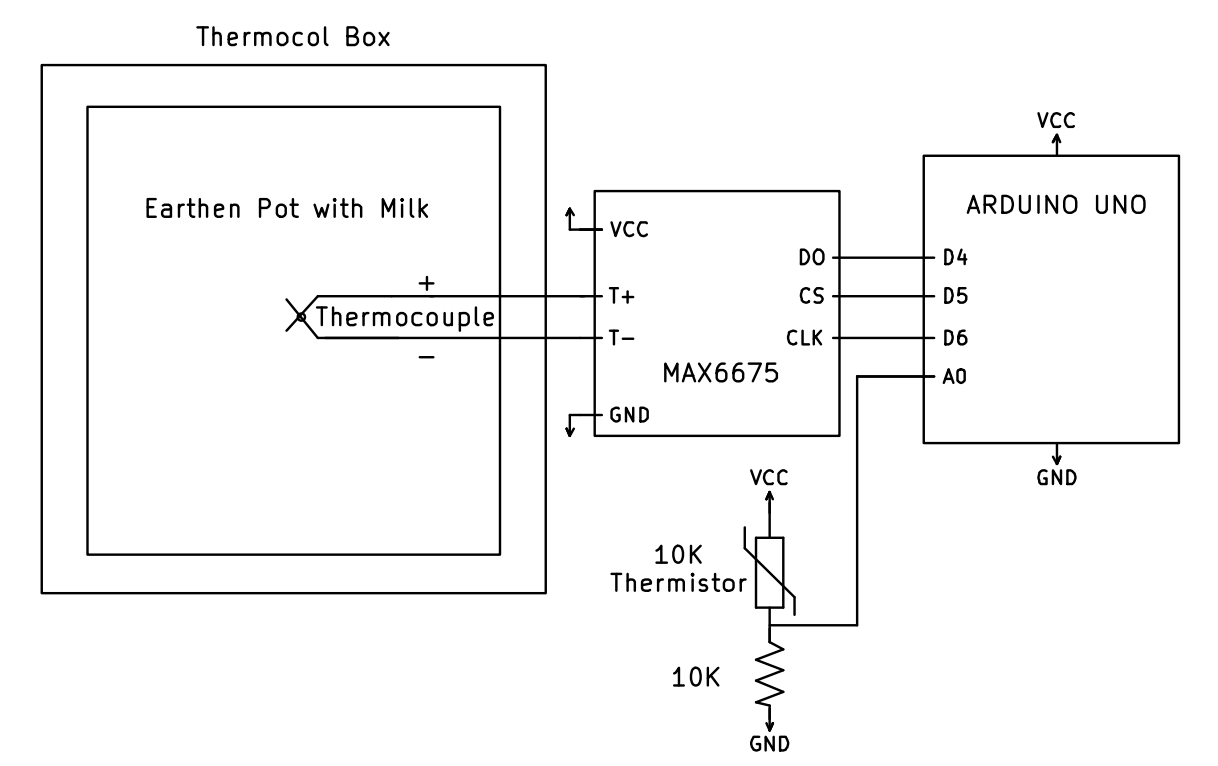
\includegraphics[width=0.8\textwidth]{images/block_diagram_1.png}}
  \caption{Temperature vs Time — Thermistor in Open}
\end{figure}
% ------------------------------



\newpage
\subsection*{Thermistor Inside Enclosure}
The thermistor inside the thermocol box exhibited smoother temperature variation with reduced external noise. This indicated that the insulation helped stabilize measurements.

\begin{figure}[H]
  \centering
  \fbox{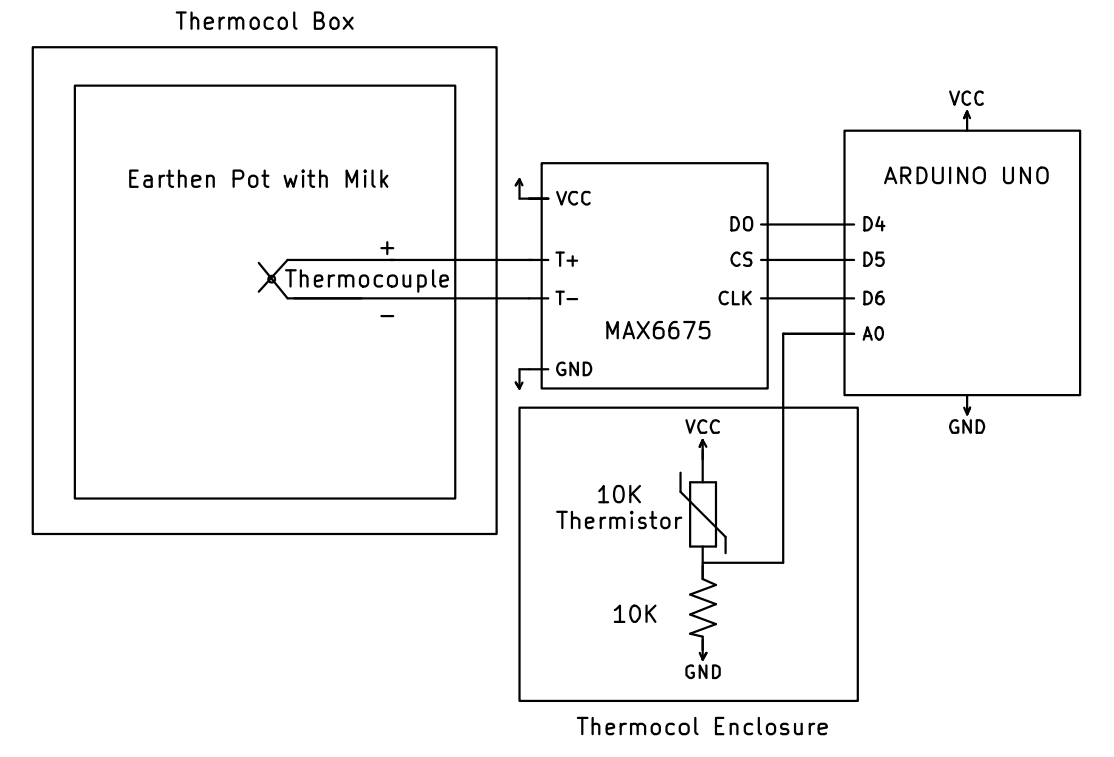
\includegraphics[width=0.8\textwidth]{images/block_diagram_2.png}}
  \caption{Temperature vs Time — Thermistor in Box}
\end{figure}


\newpage
\subsection*{Thermocouple Inside Enclosure}
The thermocouple near the milk surface recorded the actual thermal behavior during curdling. A slight dip in temperature was observed, suggesting absorption of heat consistent with an endothermic process.

\begin{figure}[H]
  \centering
  \fbox{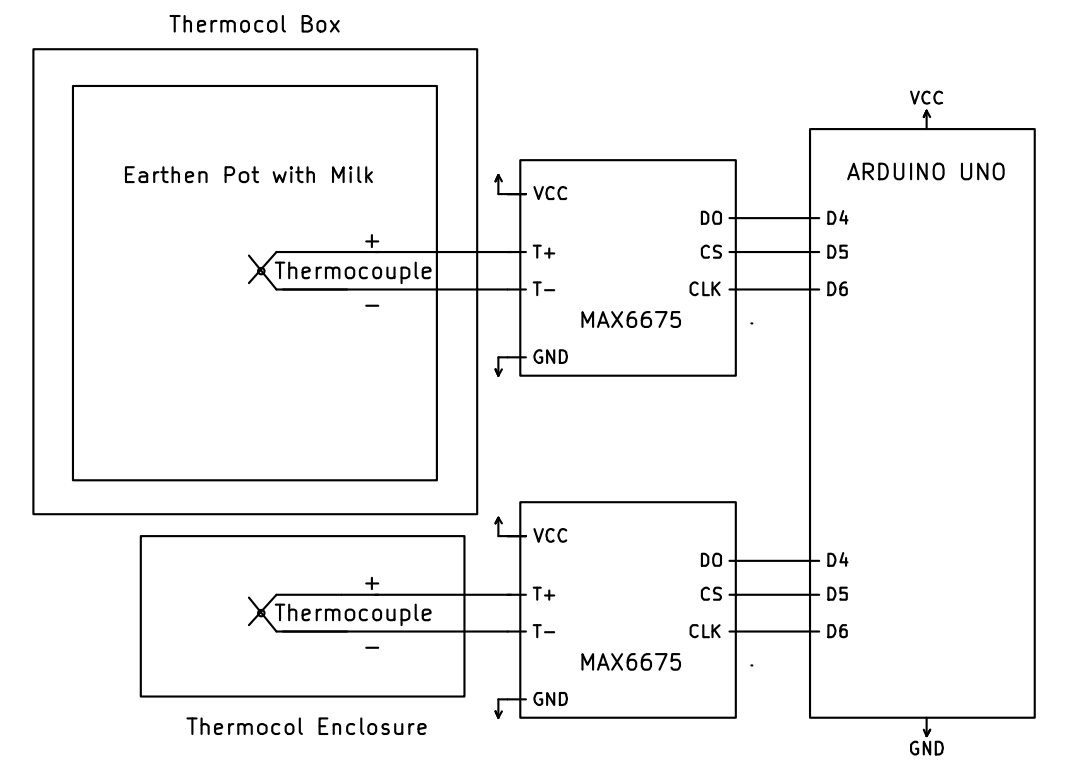
\includegraphics[width=0.8\textwidth]{images/block_diagram_3.png}}
  \caption{Temperature vs Time — Thermocouple in Box}
\end{figure}

\newpage
\section{Results}
\begin{figure}[H]
  \centering
  \fbox{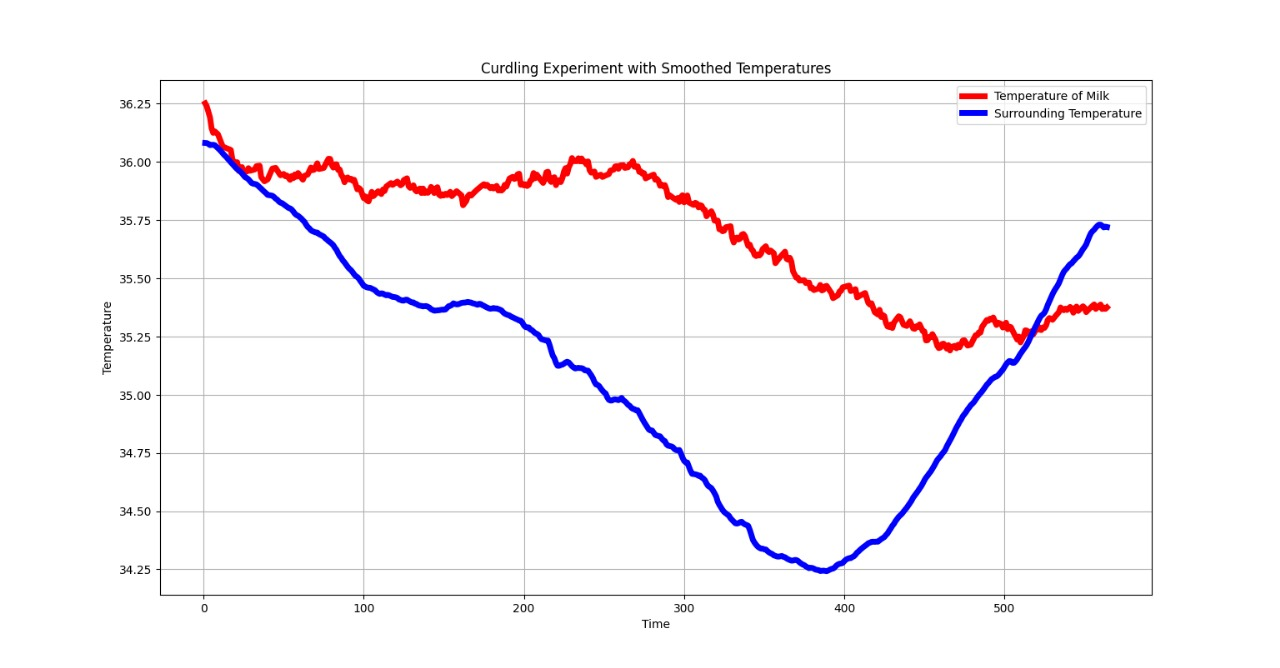
\includegraphics[width=0.8\textwidth]{images/plot_1.jpeg}}
  \caption{Temperature vs Time (Thermistor in Open Air)}
\end{figure}
During the 9-hour period, the surrounding air temperature exhibited a clear drop of nearly 2 °C, followed by recovery, while the milk temperature showed only a slight increase and decline. This thermal lag indicates that the milk absorbed heat during the process, supporting the endothermic nature of curdling.
\begin{figure}[H]
  \centering
  \fbox{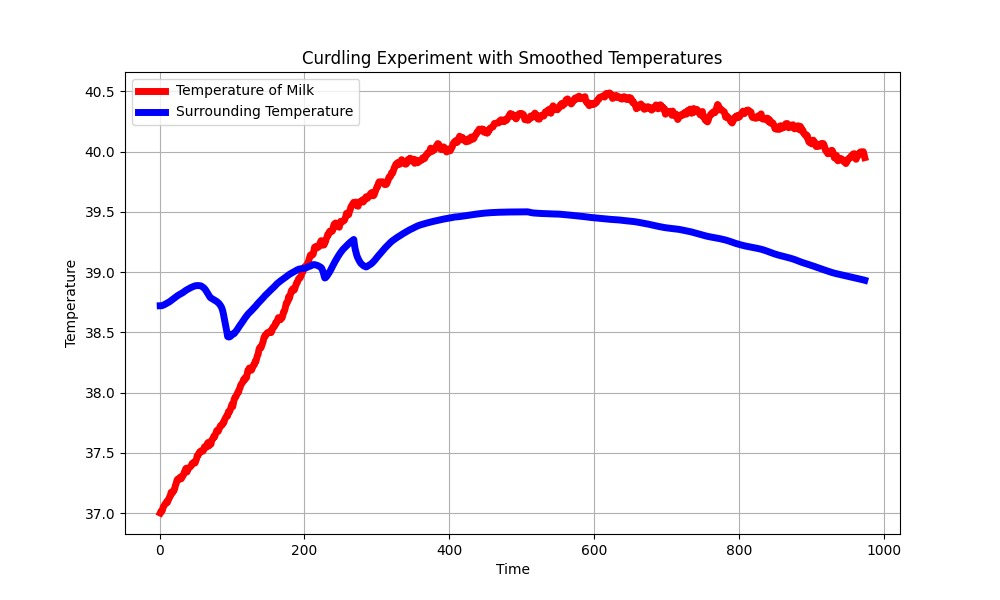
\includegraphics[width=0.8\textwidth]{images/plot_2.jpeg}}
  \caption{Temperature vs Time(Thermistor Inside Enclosure)}
\end{figure}
During 16-hour period, the milk temperature (red) increased steadily above the surroundings (blue), reaching a peak near 40.5 ° C before showing a slight decline, while the ambient temperature remained lower and more stable. The higher and sustained thermal profile of milk relative to its environment suggests continuous heat absorption, consistent with the endothermic nature of curdling.
\begin{figure}[H]
  \centering
  \fbox{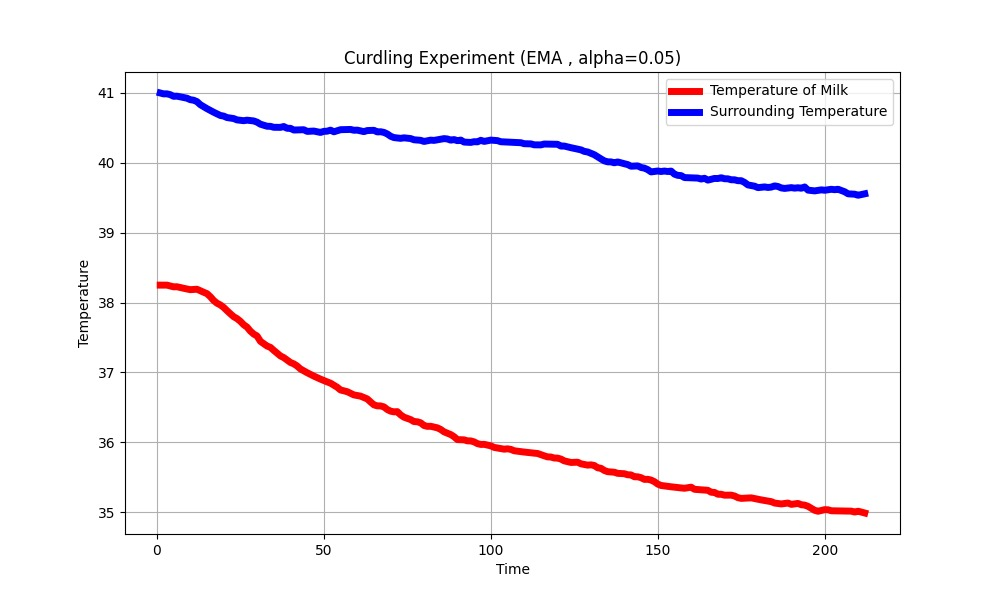
\includegraphics[width=0.8\textwidth]{images/plot_3.jpeg}}
  \caption{Temperature vs Time(Thermocouple Inside Enclosure)}
\end{figure}
During 3 hours 40 minutes, both milk and the surroundings cooled, but milk (red) showed a stronger decline, dropping nearly 3 ° C compared to the slower decrease in ambient temperature. Indicating the onset of curdling at the very start of the experiment.
\newpage
% ------------------------------
\section{Conclusion}
The experiment provided qualitative evidence suggesting curdling is an endothermic process. The sealed earthen pot showed a slight drop in temperature during the curdling period. The results, however, are not sufficient to pinpoint the exact time of curdling. For more accurate results, a pH sensor should be integrated to detect the chemical transition directly.

% ------------------------------
\section{Bill of Material}

\begin{table}[H]
\centering
\begin{tabular}{|c|l|l|c|}
\hline
\textbf{S No.} & \textbf{Component} & \textbf{Value} & \textbf{Quantity} \\ \hline
1  & Arduino Uno& & 1 \\
2 & Thermocouple( MAX6675 )& & 1\\
3 & NTC Thermistor & \SI{10}{\kilo\ohm} & 1\\
4 & Resistor & \SI{10}{\kilo\ohm} & 1 \\
5 & Earthen Pot & 500ml & 1  \\
6 & Thermocol Box & &  1  \\

\hline
\end{tabular}
\caption{Components used in the curdling experiment}
\end{table}
% ------------------------------

\section{Appendix}

\subsection*{Data File}

\begin{itemize}
  \item \href{https://drive.google.com/drive/folders/1yghCAIf9xUq-oj_R3DWdqhCwJgeraqwS?usp=sharing}{Curdling Temperature Log (CSV)}
\end{itemize}
\vspace{-5mm}
\subsection*{Code Files}
\begin{itemize}
  \item \href{https://drive.google.com/drive/folders/1wMh31OFrIGAUljoBokALCiHEpB-sdrlg?usp=drive_link}{Arduino Sketch}
\end{itemize}
\vspace{-2mm}
\begin{itemize}
  \item \href{https://drive.google.com/drive/folders/1SQ3UnZ2PInPbBjg0NKGbhzvTFUVvuViB?usp=sharing}{Python Code}
\end{itemize}
\subsection*{Arduino Libraries}
\begin{itemize}
  \item \href{https://github.com/adafruit/MAX6675-library}{MAX6675 Arduino Library by Adafruit}
\end{itemize}

\subsection*{Datasheets}
\begin{itemize}
  \item \href{https://datasheets.maximintegrated.com/en/ds/MAX6675.pdf}{MAX6675 Thermocouple Amplifier Datasheet}
   \item \href{https://docs.arduino.cc/hardware/uno-rev3/}{Arduino UNO}
  \end{itemize}
\end{document}
